\section{Практическая часть}

{\color{red} Abstract}

\subsection{Цель}

С момента своей публикации, модель Трансформера \cite{vaswani2017attention}
завоевала огромное призвание. Однако у нее есть несколько серьезных 
проблем, которые усложняют работу с длинными временным последовательностями 
(LSTF). Последующие ислледования предложили различные методы решения 
данных и связующих проблем (см. Informer \cite{informer}, Performer \cite{performer}, 
Autoformer \cite{autoformer}, PatchTST \cite{patchTST}, TFT \cite{TFT} и др.). 
В данной работе мы сфокусируемся на первых трех.

В данной работе, мы предлагаем заменить слой эмбеддинга в модели 
Informer компактным двухслойным сверточным блоком с целью повышения 
эффективности извлечения локальных паттернов, внедрить модуль 
декомпозиции ряда из Autoformer для явного разделения 
трендовых и сезонных компонент и заменить ProbSparse-внимание 
на линейное FAVOR+ из Performer для учёта глобальных 
зависимостей при низких вычислительных затратах.

\subsection{Используемые данные}

Прежде чем перейти к методологии нашей работы, рассмотрим 
модели и понятия, которыми далее будем пользоваться.

\subsubsection{Informer}

В 2021 году, Zhou et al., опубликовали свою статью 
«\textbf{Informer: Beyond Efficient Transformer for 
Long Sequence Time-Series Forecasting}», в которой 
представили новую, основанную на Трансформере \cite{vaswani2017attention} 
модель под названием \textbf{Informer} \cite{informer}. 

\begin{figure}[h!]
    \centering
    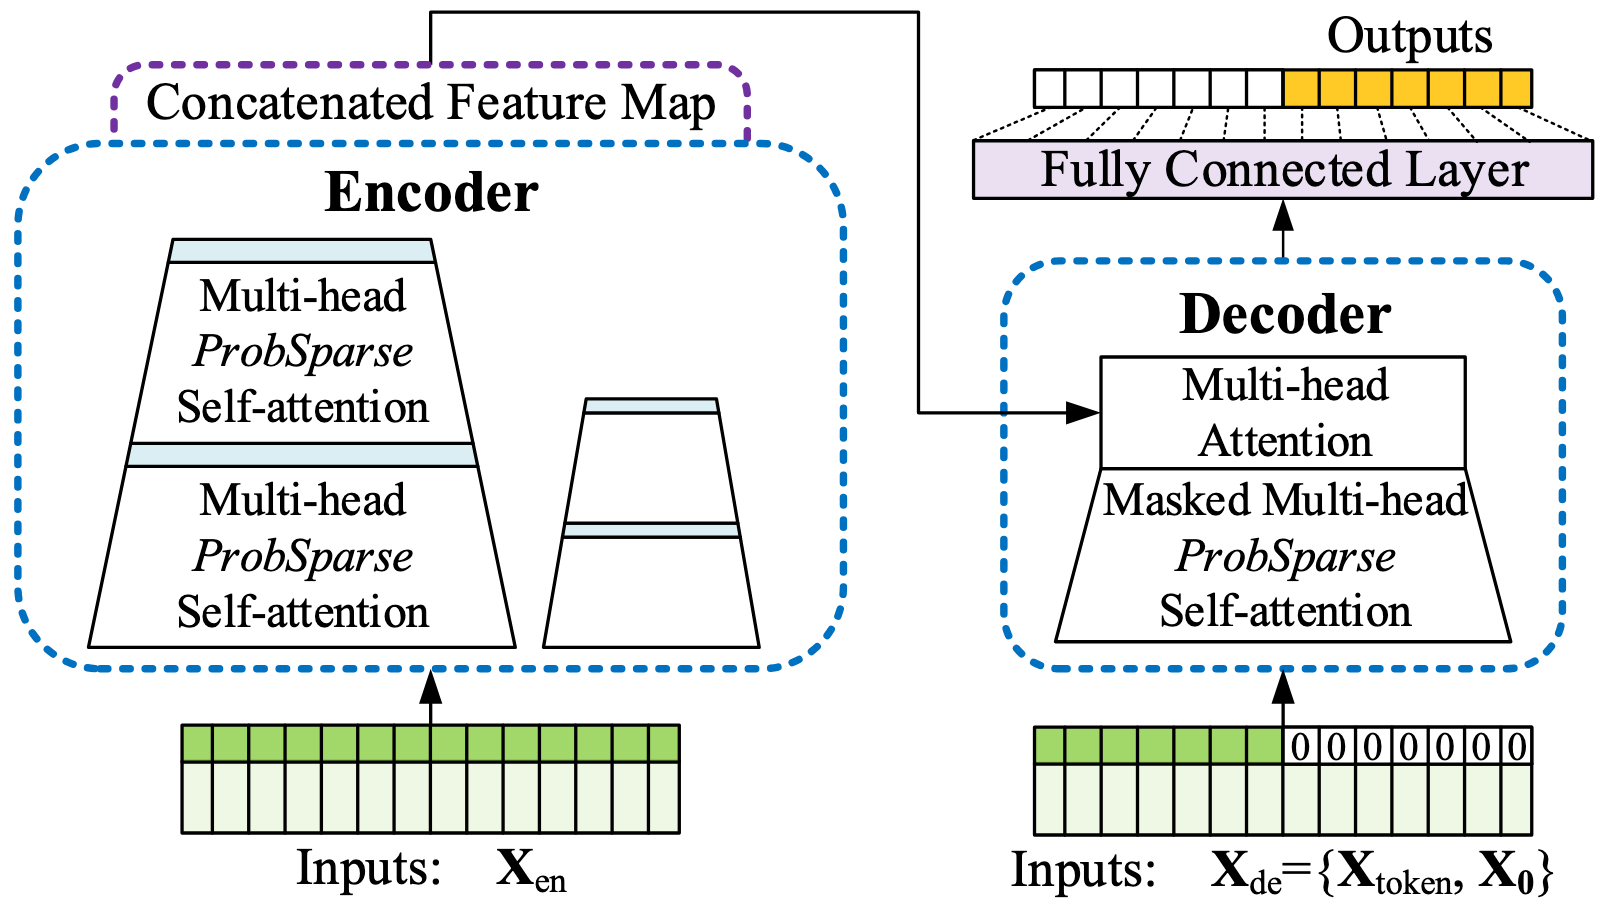
\includegraphics[width=0.8\textwidth, keepaspectratio]{informer}
    \caption{Обзор модели Informer \cite{informer}.}
    \label{fig:informer}
\end{figure}

Informer был создан для решения задачи 
\textbf{Long-sequence time-series forecasting (LSTF)}. 
Zhou et al. поставили перед собой следюущий вопрос: 
Можем ли мы построить модель, основанную на трансформере, 
которая 
\begin{enumerate}[label=(\alph*)]
    \item захватывает очень длинные зависимости
    \item эффективно работает для тысячи временных шагов
\end{enumerate}
Ключевые рассматриваемые слабости трансформера:
\begin{itemize}
    \item Квадратичная стоимость механизма само-внимания (self-attention) 
    для последовательностей длины $L$.
    \item Накладывание слоев умножает эту стоимость, достигая ограничений по памяти.
    \item Пошаговое (динамичное) декодирование работает медленно и накапливает ошибки. 
\end{itemize}

Информер отвечает на каждый из этих вопросов, реконструируя 
механизм внимания, кодировщик и декодер.

\paragraph{ProbSparse Self-Attention}

Зачастую, в длинных временных рядах, большинство 
скалярных произведений запросов с ключами пренебрежимо малы 
и лишь некоторые из них достаточно больши. 
Вместо того, чтобы считать все возможные пары запрос-ключ, 
informer предлагает следующее:
\begin{enumerate}
    \item Измерить разброс каждого запроса $q_i$:
    \begin{equation*}
        M(\bm{q}_i, \bm{K}) = \text{max}_j \cfrac{\bm{q}_i \bm{k}_j^T}{\sqrt{d}} - 
        \cfrac{1}{L_K} \sum_{j=1}^{L_K} \cfrac{\bm{q}_i \bm{k}_j^T}{sqrt{d}}, 
    \end{equation*}
    \item Выбрать $u$ лучших запросов, исходя из $M(\bm{q}_i, \bm{K})$, 
    где $u \propto \ln L$.
    \item Вычислить полное внимание только для этих $u$ рядов и 
    аппроксимировать остальные через среднее значение.
\end{enumerate}
Что сокращает как время, так и память c $O(L^2)$ до $O(L \text{log} L)$, 
при этом сохраняя всю важную информацию.

\paragraph{Self-Attention Distilling \& Кодировщик}

Даже после предыдщей операции, каждый слой все равно производит 
карты признаков длины $L$, многие из которых повторяют похожие паттерны. 
Мы можем «дистиллировать» сильнейшие сигналы и сократить последовательность 
по мере продвижения.

\begin{itemize}
    \item После каждого блока с механизмом внимания, применяем:
    \begin{enumerate}
        \item 1-D свертку + ELU активацию, 
        \item max-pool со страйдом 2 
    \end{enumerate}
\end{itemize}
Что уменьшает размерность в два раза на каждом слое, результируя 
в пирамиде стэков, чьи выходы в конечном итоге конкатенируют. 

Self-attention distilling фокусируется на доминирующих паттернах, 
при этом сокращая память до $O((2-\epsilon)L \log L)$.

\begin{figure}[h!]
    \centering
    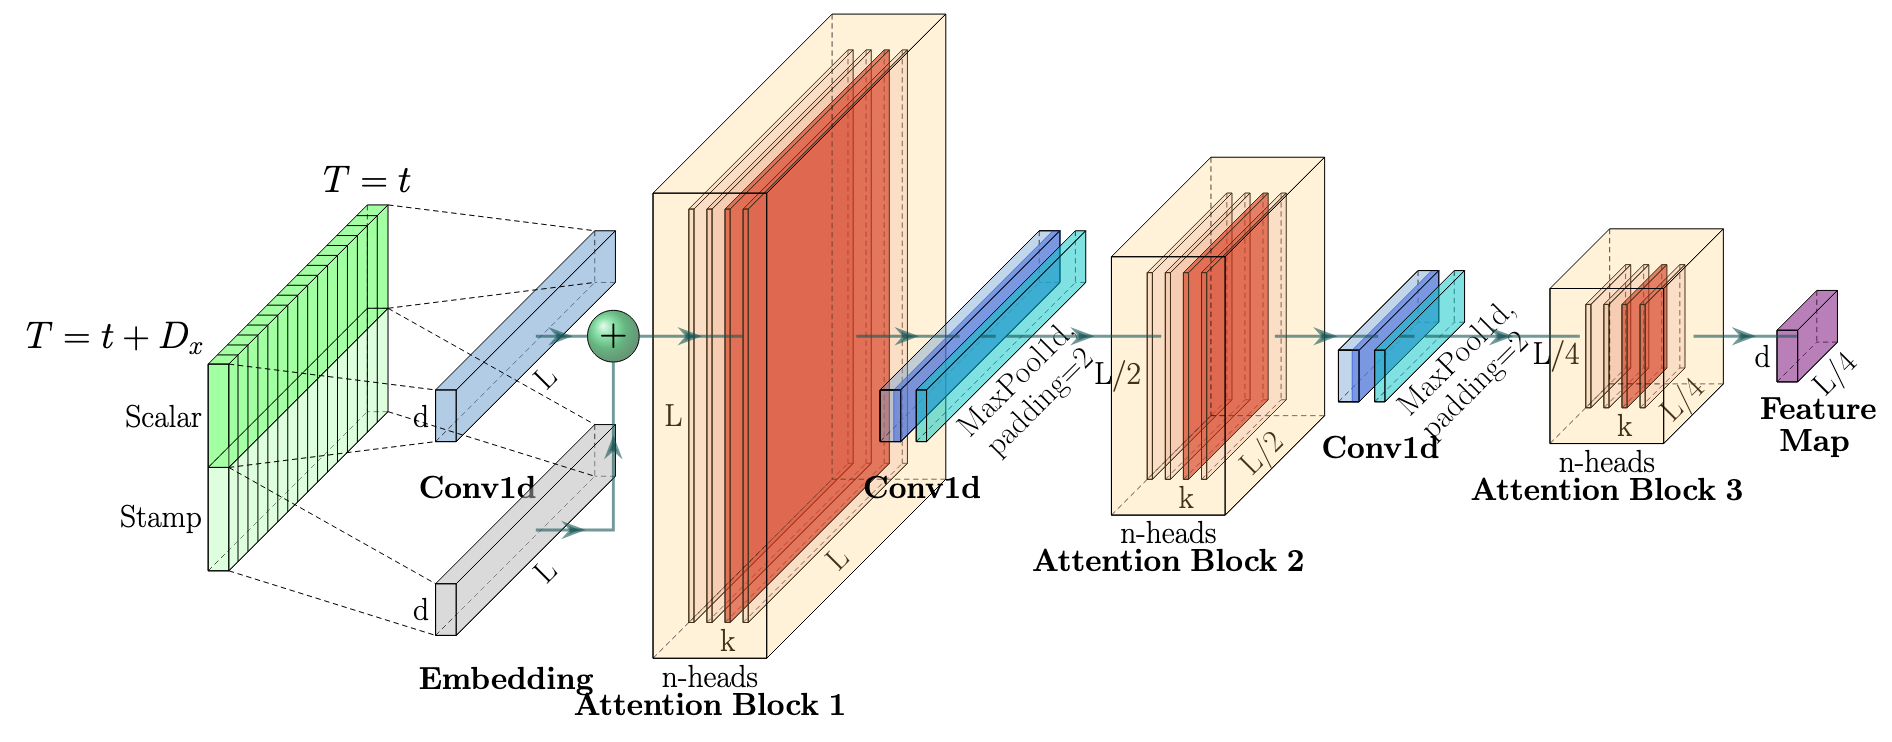
\includegraphics[width=1\textwidth, keepaspectratio]{informer_encoder}
    \caption{Обзор одного стэка в кодировщике Informer-а \cite{informer}.}
    \label{fig:informer_encoder}
\end{figure}

\paragraph{Генеративный декодер}

Вместо того, чтобы генерировать генерировать токены по очереди 
один за одним, заимствуем трюк с начальными токеном из NLP:
\begin{itemize}
    \item Взять срез ивестной истории (например 5 дней перед целевыми 7ю днями) в качесвте начального токена
    \item Разместить плейсхолдеры для всех $L_y$ будущих значение (используя только их временные метки для позиционного контекста)
    \item За один прямой проход одновременно заполнить все $L_y$ выходов через маскированное ProbSparse внимание.
\end{itemize} 
Что избегает накапливания ошибки и работает гораздо быстрее.

\subsubsection{Performer}

\subsubsection{Autoformer}

\subsection{Методология}

\subsubsection{Повышение эффективности извлечения локальных паттернов}

\subsubsection{Заимствование механизма внимания из Performer}

\subsubsection{Внедрение модуля декомпозиции ряда из Autoformer}

% put here full end architecture

\subsection{Эксперимент}

\subsubsection{Датасет}

\subsubsection{Детали}

\paragraph{Training}
\paragraph{Baselines} % compare with everything
\paragraph{Hyper-parameter tuning}
\paragraph{Setup}
\paragraph{Metrics}
\paragraph{Platform}

\subsection{Результаты}

\subsection{Заключение}

